\documentclass[12pt]{article}

% TEMPLATE DEFAULT PACKAGES
\usepackage{amssymb,amsmath,amsfonts,eurosym,geometry,ulem,graphicx,color,setspace,sectsty,comment,natbib,pdflscape,array,adjustbox}

% ADDED PACKAGES FOR THIS MANUSCRIPT
\usepackage{palatino,newtxmath,multirow,titlesec,threeparttable,tabu,booktabs,titlesec,threeparttable,mathtools,bm,bbm,subcaption,pdflscape,tcolorbox,mathrsfs}
% endfloat,

\usepackage{afterpage}
\usepackage[hyphens]{url}
\usepackage[margin=1cm]{caption}

\usepackage[draft]{hyperref}
\newcommand{\tim}{$\,\times\,$}
% FIGURES & TABLES CAPTION STYLING
\captionsetup[figure]{labelfont={bf},name={Figure},labelsep=period}
\captionsetup[table]{labelfont={bf},name={Table},labelsep=period}

% SECTION TITLE SETTINGS
\titlelabel{\thetitle.\enskip}
\titleformat*{\section}{\large\bfseries}
\titleformat*{\subsection}{\normalsize\bfseries}

% COLUMN TYPES
\newcolumntype{L}[1]{>{\raggedright\let\newline\\\arraybackslash\hspace{0pt}}m{#1}}
\newcolumntype{C}{>{\centering\arraybackslash}p{5.2em}}
\newcolumntype{D}{>{\centering\arraybackslash}p{5em}}
\newcolumntype{R}[1]{>{\raggedleft\let\newline\\\arraybackslash\hspace{0pt}}m{#1}}


% MARGINS AND SPACING
\normalem
\geometry{left=1.1in,right=1.1in,top=1.0in,bottom=1.0in}
\setlength{\parskip}{2.5pt}

% SPECIAL CELL 
\newcommand{\specialcell}[2][c]{%
	\begin{tabular}[#1]{@{}l@{}}#2\end{tabular}}

% NO INDENT ON FOOTNOTES
\usepackage[hang,flushmargin]{footmisc}

\begin{document}



\vspace{0mm}
\begin{table}[h!]
\centering
\caption{Housing Project Areas Description}\label{table:projectdescriptives}
\vspace{0mm}
\begin{tabular}{l*{1}{cccccc}}
\toprule
  & \multicolumn{2}{c}{\textbf{All}}& \multicolumn{2}{c}{\textbf{Greenfield}}  & \multicolumn{2}{c}{\textbf{In-Situ}}   \\
  &Const. & Unconst. &Const. & Unconst.   & Const. & Unconst. \\
\midrule
 Number of Projects  & 172  & 145  & 43  & 20  & 27  & 29  \\ 
 Area (km2)  & 1.17  & 1.16  & 1.72  & 2.42  & 1.50  & 0.88  \\ 
 Median Construction Yr.  & 2006  & 2006  & 2006  & 2005  & 2004  & 2006  \\ 
 Delivered Houses  & 374  & 11  & 568  & 24  & 702  & 20  \\ 
 House Price in 1 km (R$^\dagger$)  & 188,441  & 218,635  & 194,214  & 186,841  & 179,596  & 208,570  \\ 
 Distance to CBD$^\ddagger$ (km)  & 32.5  & 27.7  & 40.5  & 39.9  & 32.6  & 30.6  \\ 

\bottomrule
\multicolumn{7}{l}{\scriptsize Const. refers to constructed projects and unconst. refers to unconstructed projects.}\\[-.5em]
\multicolumn{7}{l}{\scriptsize $^*$Calculated from {\it expected} completion dates using Gauteng National Treasury budget reports.}\\[-.5em]
\multicolumn{7}{l}{\scriptsize $^\dagger$ The USD averaged to about 7.70 Rands during the 2001-2011 period.}\\[-.5em]
\multicolumn{7}{l}{\scriptsize $^\ddagger$Measured as the average minimum distance with respect to Johannesburg and Pretoria CBDs. } \\[-.5em]
%\multicolumn{7}{l}{\scriptsize City includes projects whose centroids are within 30.4 km of their nearest CBD.} \\[-.5em]
%\multicolumn{7}{l}{\scriptsize Suburb includes projects whose centroids are further than 30.4 km from their nearest CBD.}
\end{tabular}
\end{table} 



\begin{figure*}
        \centering
   %     \caption[ Pre-Period Housing Densities in Constructed and Unconstructed Projects Areas ]
  %      {\small Pre-Period Densities} 
        %\vspace{2mm}
        \begin{subfigure}[b]{0.48\textwidth}
                    \caption[Network2]%
            {{\footnotesize \textbf{All Projects} pre-period formal raw data}}    
            \label{fig:prefor}
            \centering
            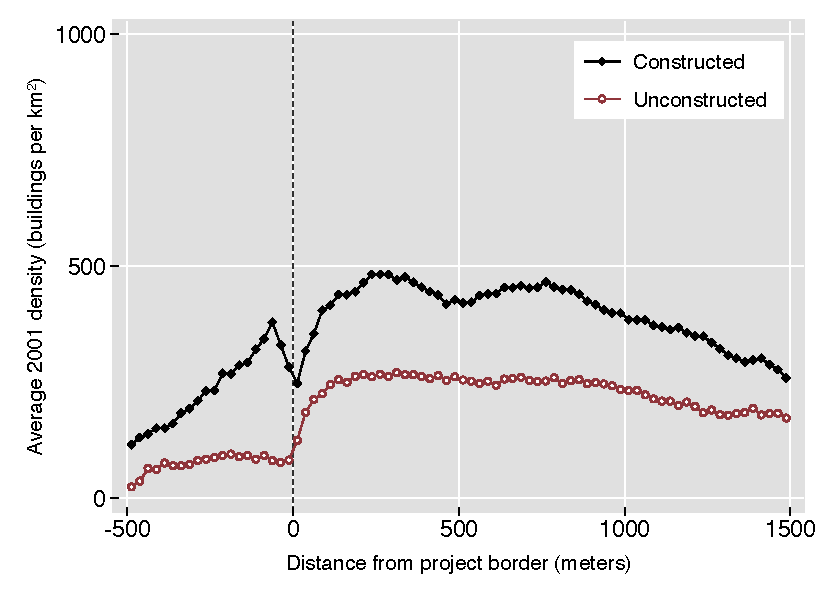
\includegraphics[width=\textwidth,trim={0.3cm .3cm 0.1cm 0cm}, clip=true]{figures/bblu_for_pre_means_4_spk.pdf}

        \end{subfigure}
        \hfill
        \begin{subfigure}[b]{0.48\textwidth}  
                    \caption[]%
            {{\footnotesize \textbf{All Projects} pre-period informal  raw data}}      
            \label{fig:preinf}
            \centering 
            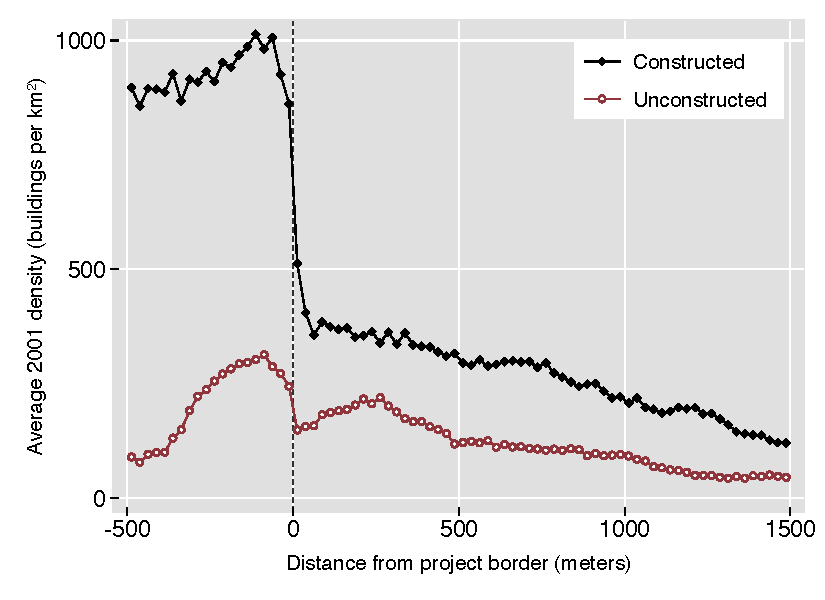
\includegraphics[width=\textwidth,trim={0.3cm .3cm 0.1cm 0cm}, clip=true]{figures/bblu_inf_pre_means_4_spk.pdf}

        \end{subfigure}
        \begin{subfigure}[b]{0.48\textwidth}
                    \caption[Network2]%
            {{\footnotesize \textbf{Greenfield} pre-period formal  raw data}}    
            \label{fig:prefor}
            \centering
            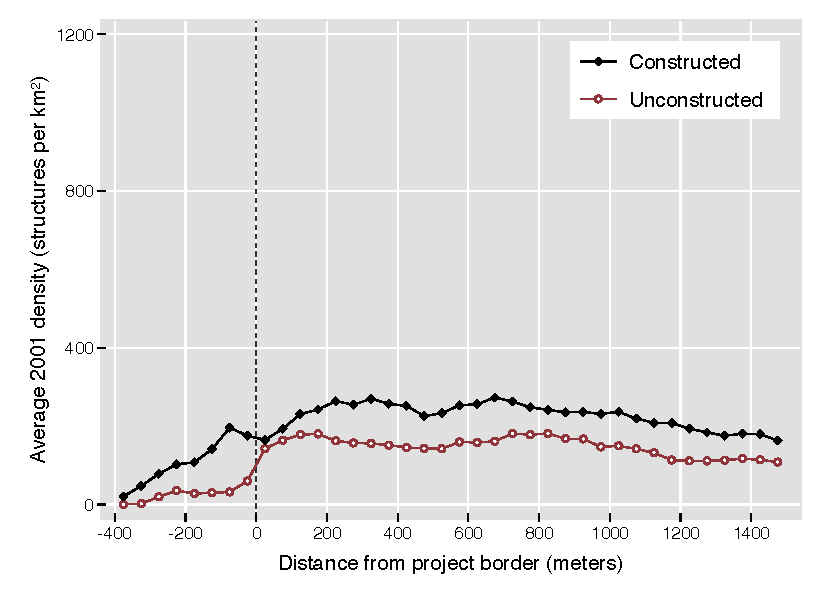
\includegraphics[width=\textwidth,trim={0.3cm .3cm 0.1cm 0cm}, clip=true]{figures/bblu_for_pre_means_4_1_spk.pdf}

        \end{subfigure}
        \hfill
        \begin{subfigure}[b]{0.48\textwidth}  
                    \caption[]%
            {{\footnotesize \textbf{Greenfield} pre-period informal  raw data}}     
            \label{fig:preinf}
            \centering 
            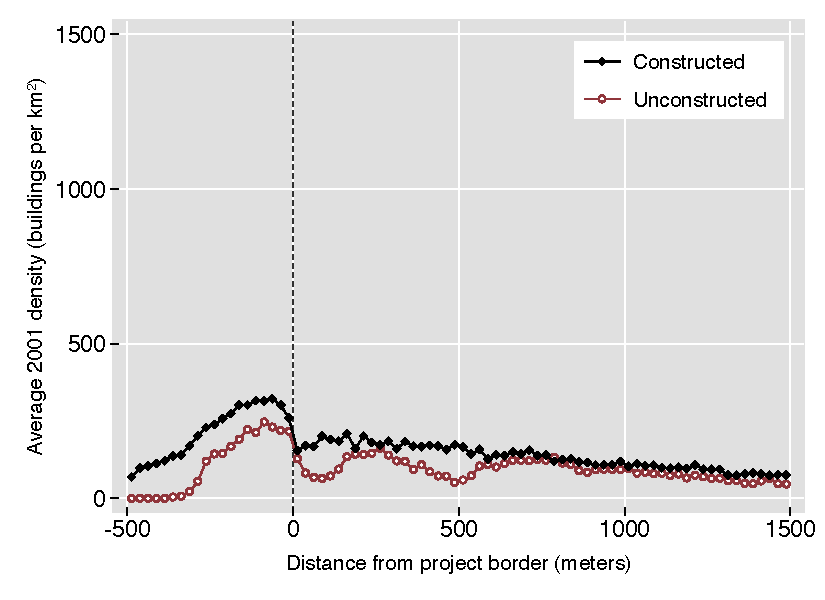
\includegraphics[width=\textwidth,trim={0.3cm .3cm 0.1cm 0cm}, clip=true]{figures/bblu_inf_pre_means_4_1_spk.pdf}

        \end{subfigure}
        \begin{subfigure}[b]{0.48\textwidth}
                    \caption[Network2]%
            {{\footnotesize \textbf{In-Situ} pre-period formal  raw data}}   
            \label{fig:prefor}
            \centering
            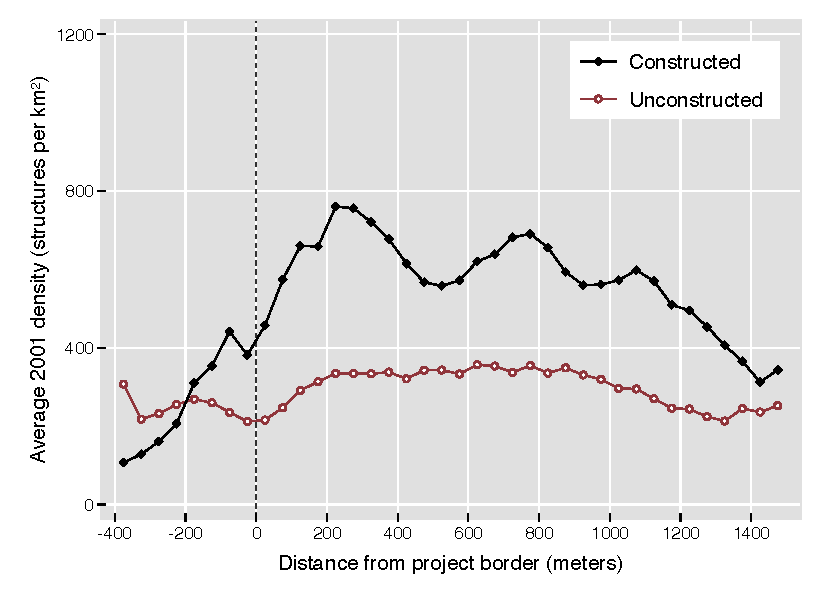
\includegraphics[width=\textwidth,trim={0.3cm .3cm 0.1cm 0cm}, clip=true]{figures/bblu_for_pre_means_4_2_spk.pdf}

        \end{subfigure}
        \hfill
        \begin{subfigure}[b]{0.48\textwidth}  
                    \caption[]%
            {{\footnotesize \textbf{In-Situ} pre-period informal  raw data}}     
            \label{fig:preinf}
            \centering 
            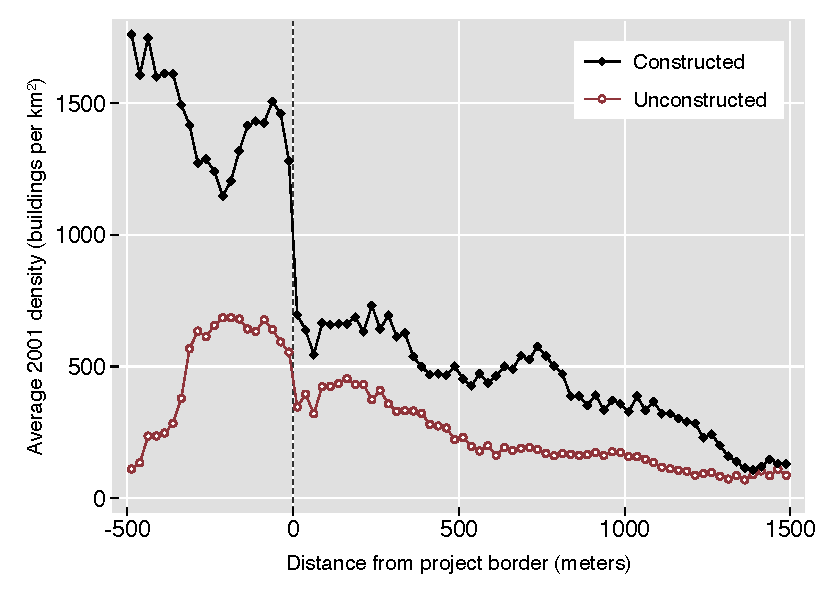
\includegraphics[width=\textwidth,trim={0.3cm .3cm 0.1cm 0cm}, clip=true]{figures/bblu_inf_pre_means_4_2_spk.pdf}

        \end{subfigure}
        \begin{subfigure}[b]{0.48\textwidth}
                    \caption[Network2]%
            {{\footnotesize \textbf{Other} pre-period formal  raw data}}   
            \label{fig:prefor}
            \centering
            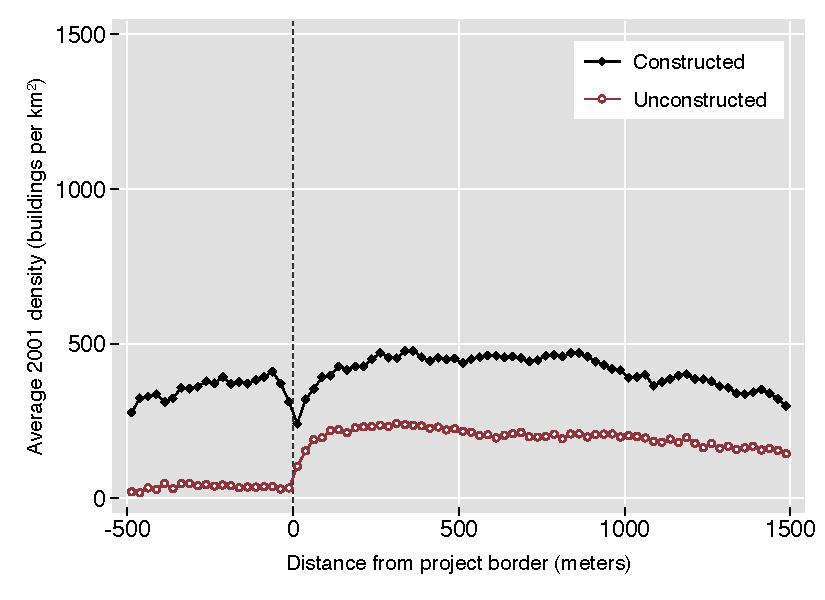
\includegraphics[width=\textwidth,trim={0.3cm .3cm 0.1cm 0cm}, clip=true]{figures/bblu_for_pre_means_4_3_spk.pdf}

        \end{subfigure}
        \hfill
        \begin{subfigure}[b]{0.48\textwidth}  
                    \caption[]%
            {{\footnotesize \textbf{Other} pre-period informal  raw data}}      
            \label{fig:preinf}
            \centering 
            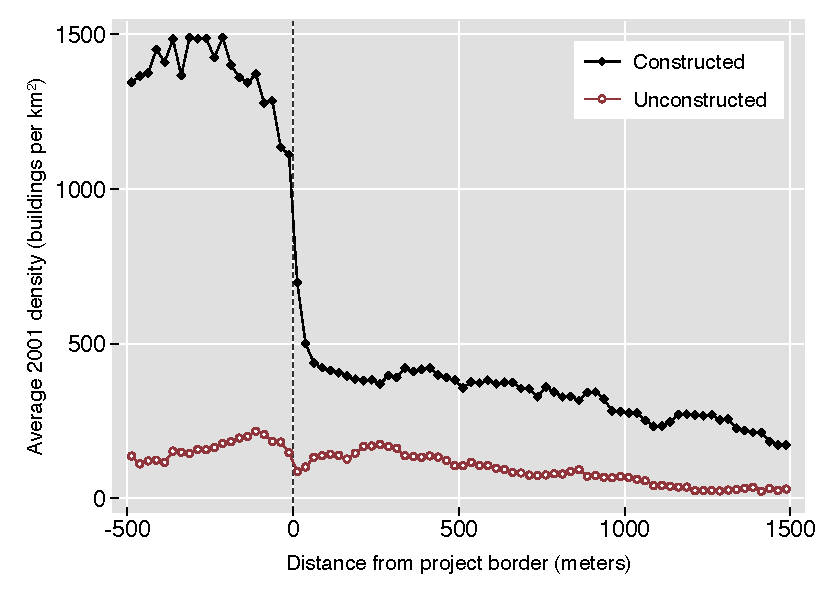
\includegraphics[width=\textwidth,trim={0.3cm .3cm 0.1cm 0cm}, clip=true]{figures/bblu_inf_pre_means_4_3_spk.pdf}

        \end{subfigure}
\end{figure*}


\begin{figure*}
        \centering
   %     \caption[ Pre-Period Housing Densities in Constructed and Unconstructed Projects Areas ]
  %      {\small Pre-Period Densities} 
        %\vspace{2mm}
        \begin{subfigure}[b]{0.48\textwidth}
                    \caption[Network2]%
            {{\footnotesize \textbf{All Projects} pre-period formal fe}}    
            \label{fig:prefor}
            \centering
            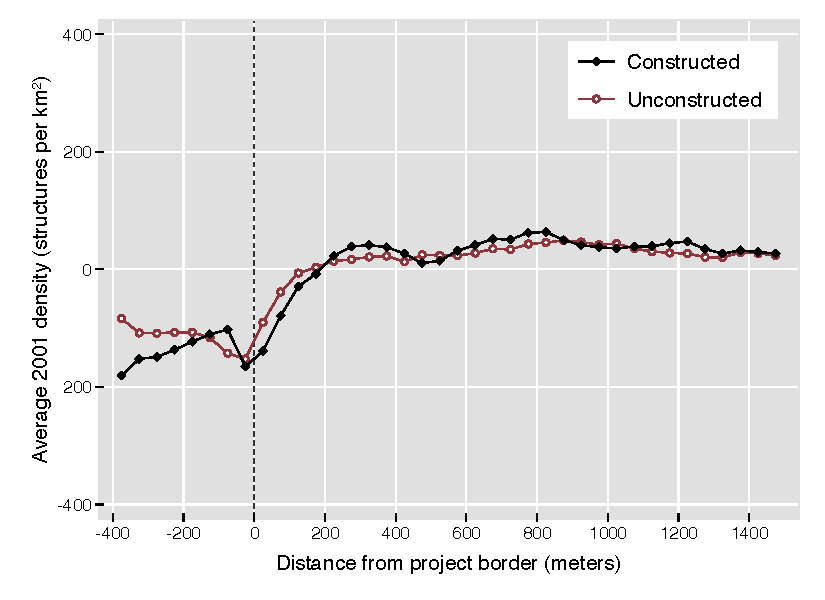
\includegraphics[width=\textwidth,trim={0.3cm .3cm 0.1cm 0cm}, clip=true]{figures/bblu_for_fe_pre_means_4_mp_postk.pdf}

        \end{subfigure}
        \hfill
        \begin{subfigure}[b]{0.48\textwidth}  
                    \caption[]%
            {{\footnotesize \textbf{All Projects} pre-period informal fe }}      
            \label{fig:preinf}
            \centering 
            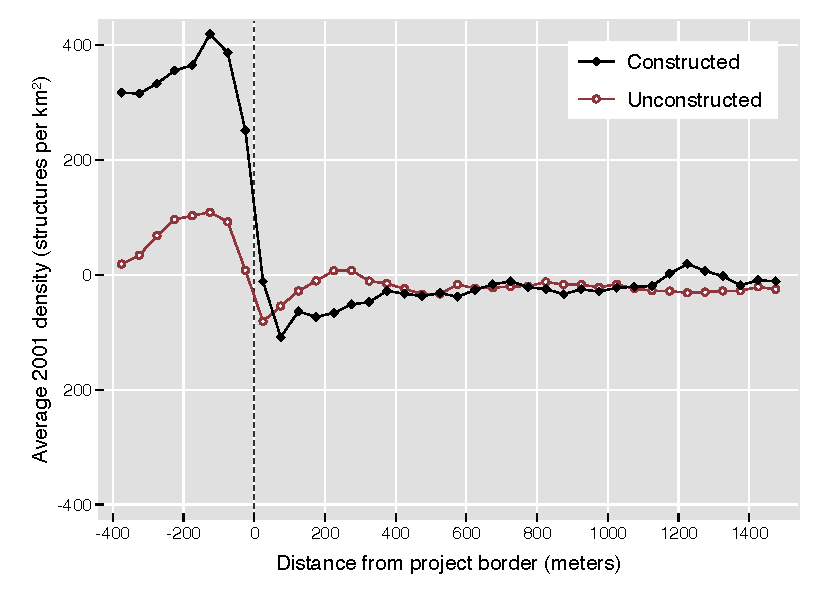
\includegraphics[width=\textwidth,trim={0.3cm .3cm 0.1cm 0cm}, clip=true]{figures/bblu_inf_fe_pre_means_4_mp_postk.pdf}

        \end{subfigure}
        \begin{subfigure}[b]{0.48\textwidth}
                    \caption[Network2]%
            {{\footnotesize \textbf{Greenfield} pre-period formal  fe }}    
            \label{fig:prefor}
            \centering
            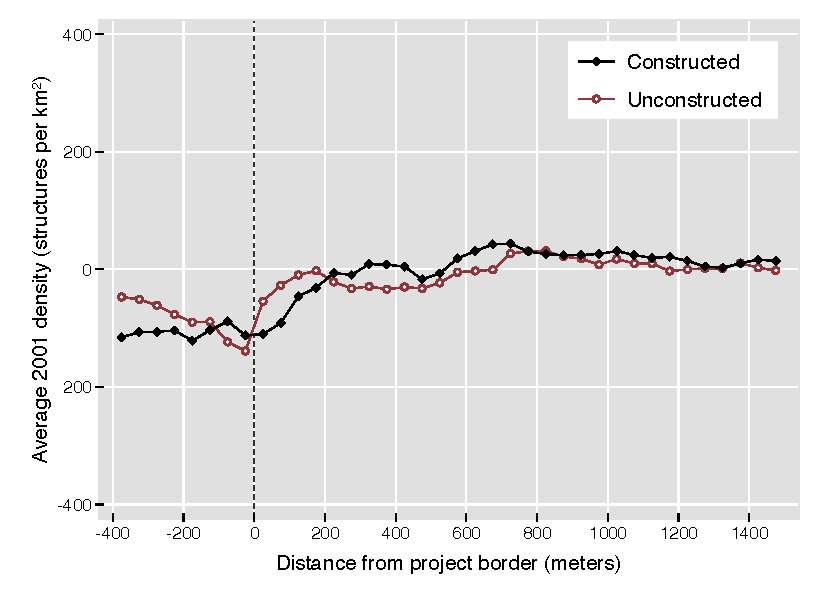
\includegraphics[width=\textwidth,trim={0.3cm .3cm 0.1cm 0cm}, clip=true]{figures/bblu_for_fe_pre_means_4_1_mp_postk.pdf}

        \end{subfigure}
        \hfill
        \begin{subfigure}[b]{0.48\textwidth}  
                    \caption[]%
            {{\footnotesize \textbf{Greenfield} pre-period informal fe }}     
            \label{fig:preinf}
            \centering 
            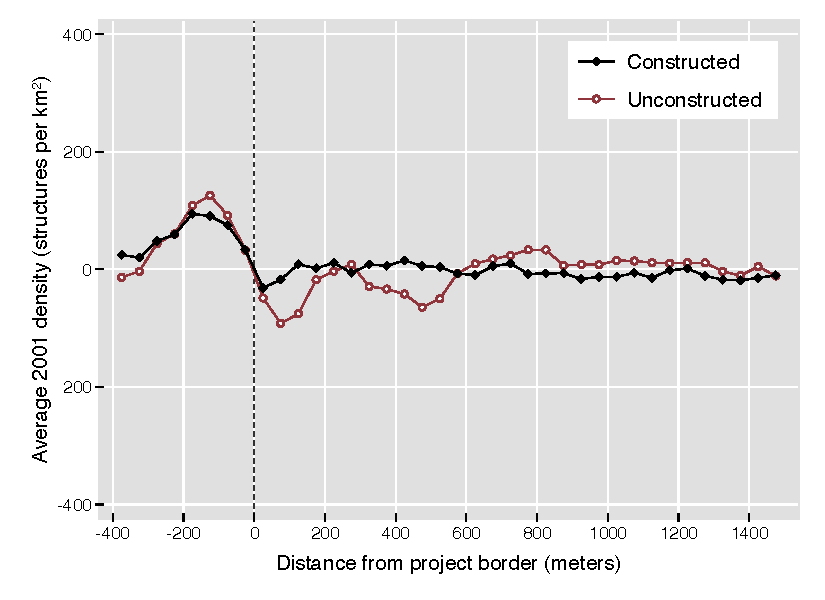
\includegraphics[width=\textwidth,trim={0.3cm .3cm 0.1cm 0cm}, clip=true]{figures/bblu_inf_fe_pre_means_4_1_mp_postk.pdf}

        \end{subfigure}
        \begin{subfigure}[b]{0.48\textwidth}
                    \caption[Network2]%
            {{\footnotesize \textbf{In-Situ} pre-period formal fe }}   
            \label{fig:prefor}
            \centering
            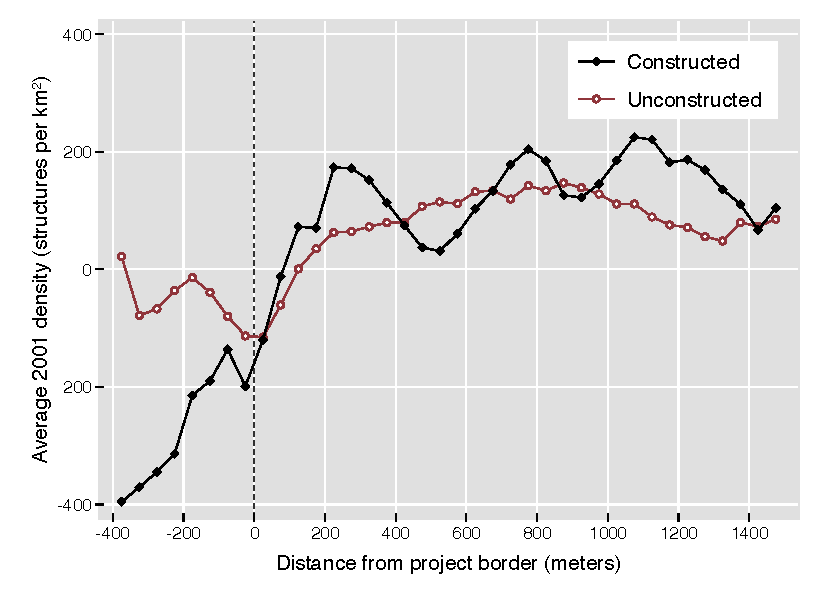
\includegraphics[width=\textwidth,trim={0.3cm .3cm 0.1cm 0cm}, clip=true]{figures/bblu_for_fe_pre_means_4_2_mp_postk.pdf}

        \end{subfigure}
        \hfill
        \begin{subfigure}[b]{0.48\textwidth}  
                    \caption[]%
            {{\footnotesize \textbf{In-Situ} pre-period informal fe }}     
            \label{fig:preinf}
            \centering 
            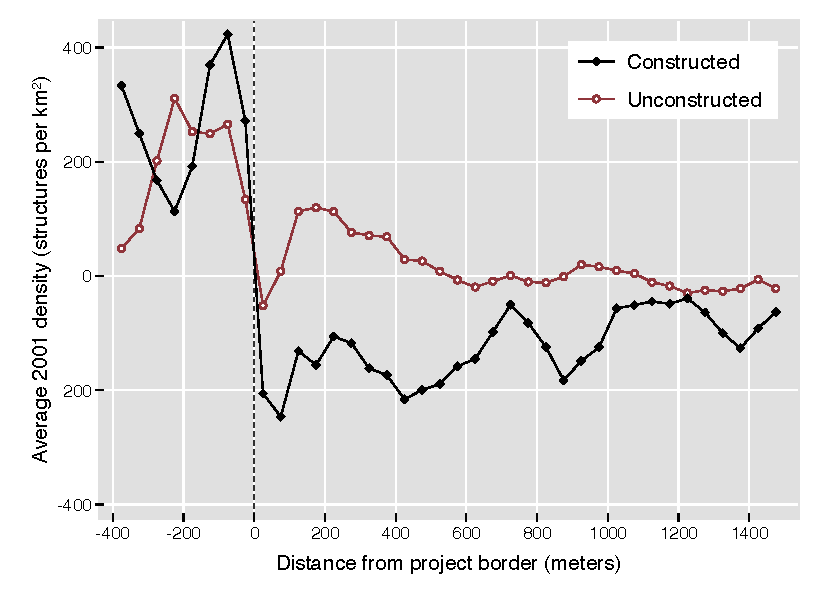
\includegraphics[width=\textwidth,trim={0.3cm .3cm 0.1cm 0cm}, clip=true]{figures/bblu_inf_fe_pre_means_4_2_mp_postk.pdf}

        \end{subfigure}
        \begin{subfigure}[b]{0.48\textwidth}
                    \caption[Network2]%
            {{\footnotesize \textbf{Other} pre-period formal fe }}   
            \label{fig:prefor}
            \centering
            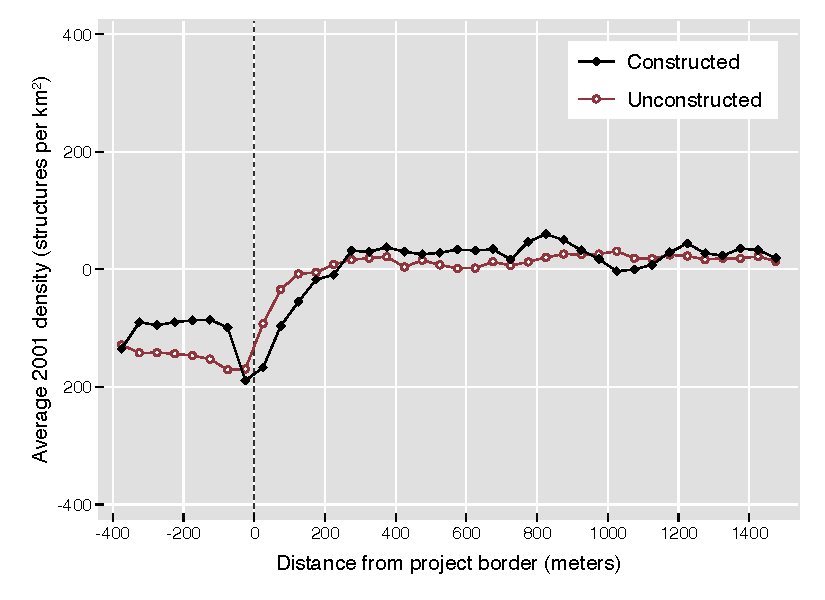
\includegraphics[width=\textwidth,trim={0.3cm .3cm 0.1cm 0cm}, clip=true]{figures/bblu_for_fe_pre_means_4_3_mp_postk.pdf}

        \end{subfigure}
        \hfill
        \begin{subfigure}[b]{0.48\textwidth}  
                    \caption[]%
            {{\footnotesize \textbf{Other} pre-period informal fe }}      
            \label{fig:preinf}
            \centering 
            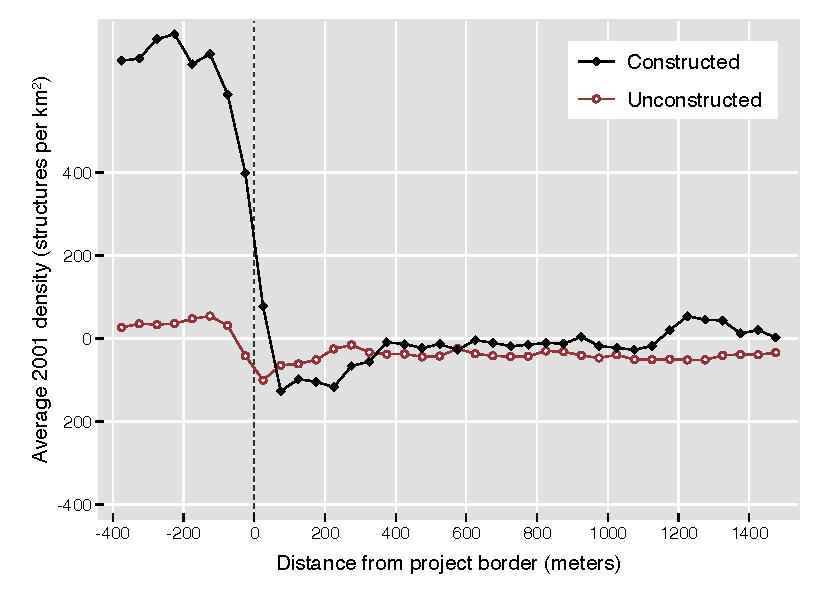
\includegraphics[width=\textwidth,trim={0.3cm .3cm 0.1cm 0cm}, clip=true]{figures/bblu_inf_fe_pre_means_4_3_mp_postk.pdf}

        \end{subfigure}
\end{figure*}








\begin{figure*}
        \centering
   %     \caption[ Pre-Period Housing Densities in Constructed and Unconstructed Projects Areas ]
  %      {\small Pre-Period Densities} 
        %\vspace{2mm}
        \begin{subfigure}[b]{0.48\textwidth}
            \caption[Network2]%
            {{\footnotesize \textbf{All Projects} changes formal raw data}}    
            \label{fig:prefor}
            \centering
            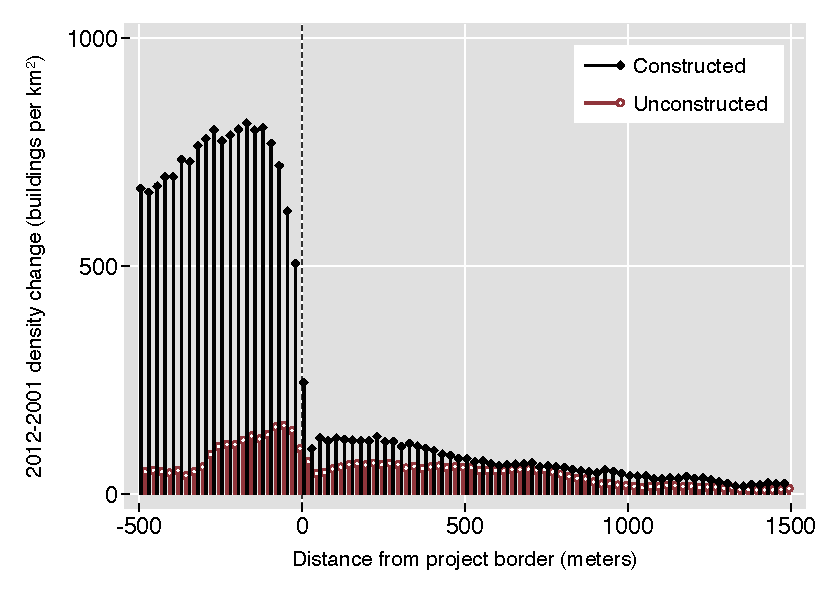
\includegraphics[width=\textwidth,trim={0.3cm .3cm 0.1cm 0cm}, clip=true]{figures/bblu_for_rawchanges_4_spk.pdf}

        \end{subfigure}
        \hfill
        \begin{subfigure}[b]{0.48\textwidth}  
                    \caption[]%
            {{\footnotesize \textbf{All Projects} changes informal  raw data}}      
            \label{fig:preinf}
            \centering 
            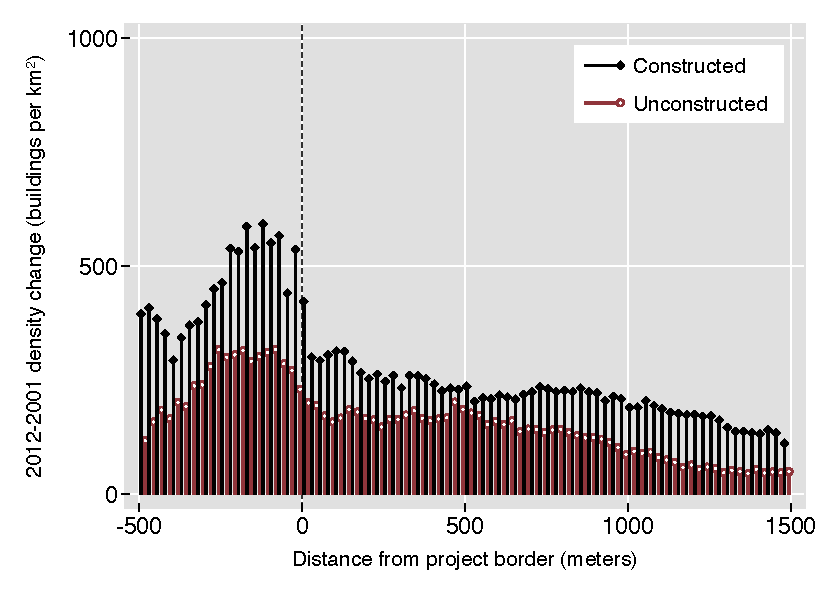
\includegraphics[width=\textwidth,trim={0.3cm .3cm 0.1cm 0cm}, clip=true]{figures/bblu_inf_rawchanges_4_spk.pdf}

        \end{subfigure}
        \begin{subfigure}[b]{0.48\textwidth}
                    \caption[Network2]%
            {{\footnotesize \textbf{Greenfield} changes formal  raw data}}    
            \label{fig:prefor}
            \centering
            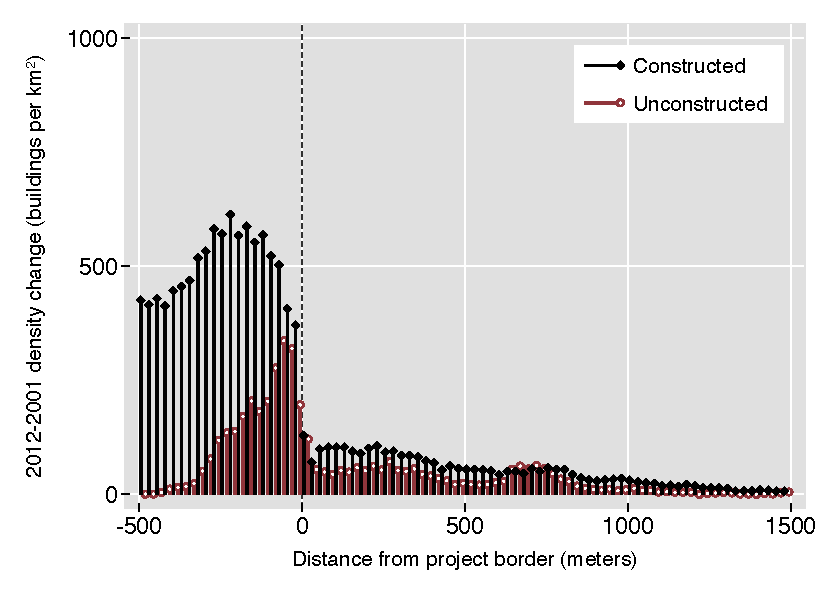
\includegraphics[width=\textwidth,trim={0.3cm .3cm 0.1cm 0cm}, clip=true]{figures/bblu_for_rawchanges_4_1_spk.pdf}

        \end{subfigure}
        \hfill
        \begin{subfigure}[b]{0.48\textwidth}  
                    \caption[]%
            {{\footnotesize \textbf{Greenfield} changes informal raw data }}     
            \label{fig:preinf}
            \centering 
            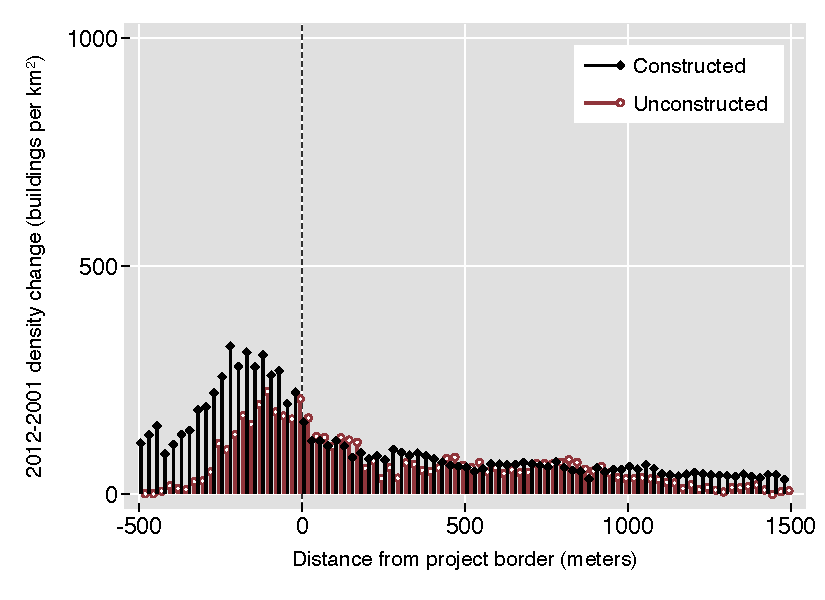
\includegraphics[width=\textwidth,trim={0.3cm .3cm 0.1cm 0cm}, clip=true]{figures/bblu_inf_rawchanges_4_1_spk.pdf}

        \end{subfigure}
        \begin{subfigure}[b]{0.48\textwidth}
                    \caption[Network2]%
            {{\footnotesize \textbf{In-Situ} changes formal raw data }}   
            \label{fig:prefor}
            \centering
            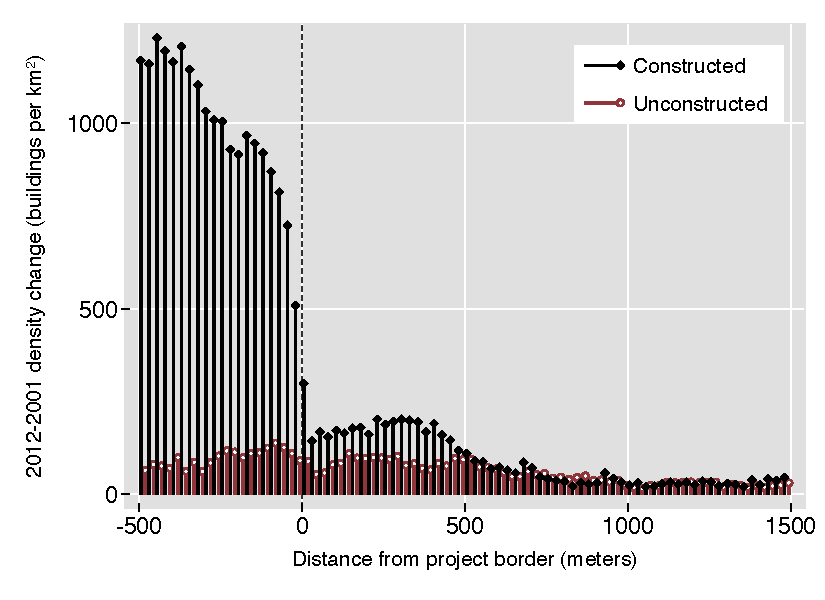
\includegraphics[width=\textwidth,trim={0.3cm .3cm 0.1cm 0cm}, clip=true]{figures/bblu_for_rawchanges_4_2_spk.pdf}

        \end{subfigure}
        \hfill
        \begin{subfigure}[b]{0.48\textwidth}  
                    \caption[]%
            {{\footnotesize \textbf{In-Situ} changes informal raw data }}     
            \label{fig:preinf}
            \centering 
            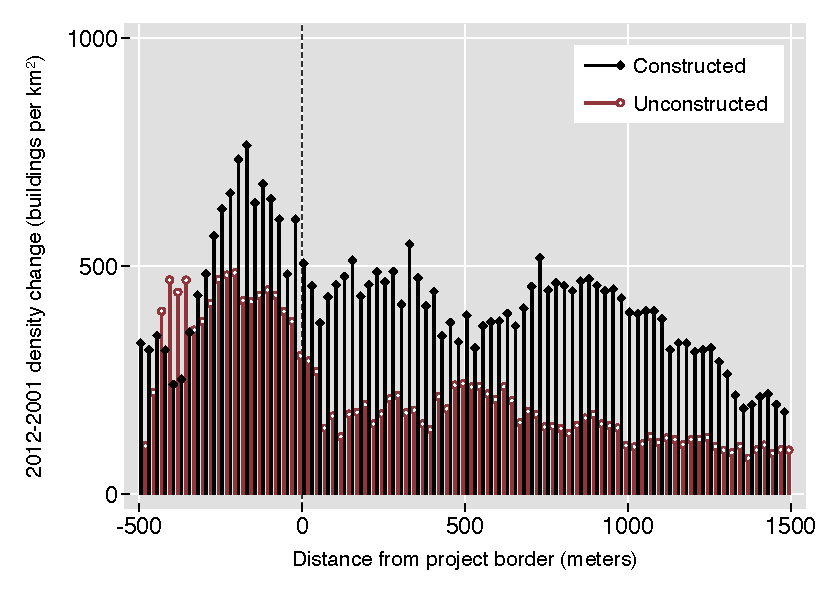
\includegraphics[width=\textwidth,trim={0.3cm .3cm 0.1cm 0cm}, clip=true]{figures/bblu_inf_rawchanges_4_2_spk.pdf}

        \end{subfigure}
        \begin{subfigure}[b]{0.48\textwidth}
                    \caption[Network2]%
            {{\footnotesize \textbf{Other} changes formal raw data}}   
            \label{fig:prefor}
            \centering
            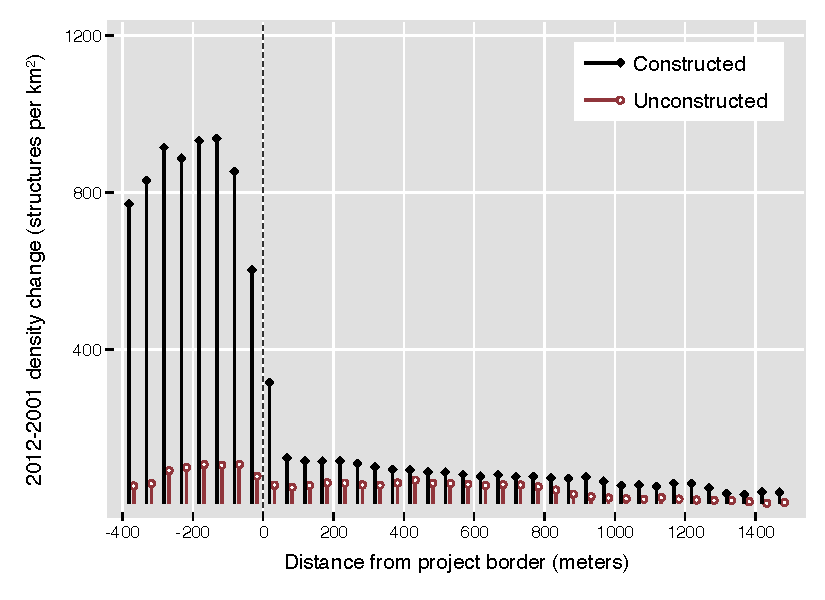
\includegraphics[width=\textwidth,trim={0.3cm .3cm 0.1cm 0cm}, clip=true]{figures/bblu_for_rawchanges_4_3_spk.pdf}

        \end{subfigure}
        \hfill
        \begin{subfigure}[b]{0.48\textwidth} 
                    \caption[]%
            {{\footnotesize \textbf{Other} changes informal  raw data}}      
            \label{fig:preinf} 
            \centering 
            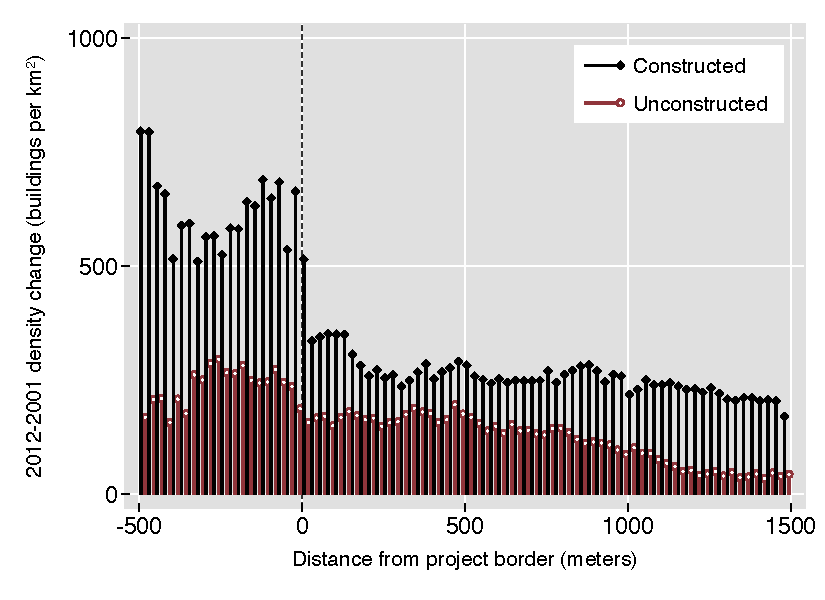
\includegraphics[width=\textwidth,trim={0.3cm .3cm 0.1cm 0cm}, clip=true]{figures/bblu_inf_rawchanges_4_3_spk.pdf}

        \end{subfigure}
\end{figure*}




\begin{figure*}
        \centering
   %     \caption[ Pre-Period Housing Densities in Constructed and Unconstructed Projects Areas ]
  %      {\small Pre-Period Densities} 
        %\vspace{2mm}
        \begin{subfigure}[b]{0.48\textwidth}
            \caption[Network2]%
            {{\footnotesize \textbf{All Projects} changes formal fe }}    
            \label{fig:prefor}
            \centering
            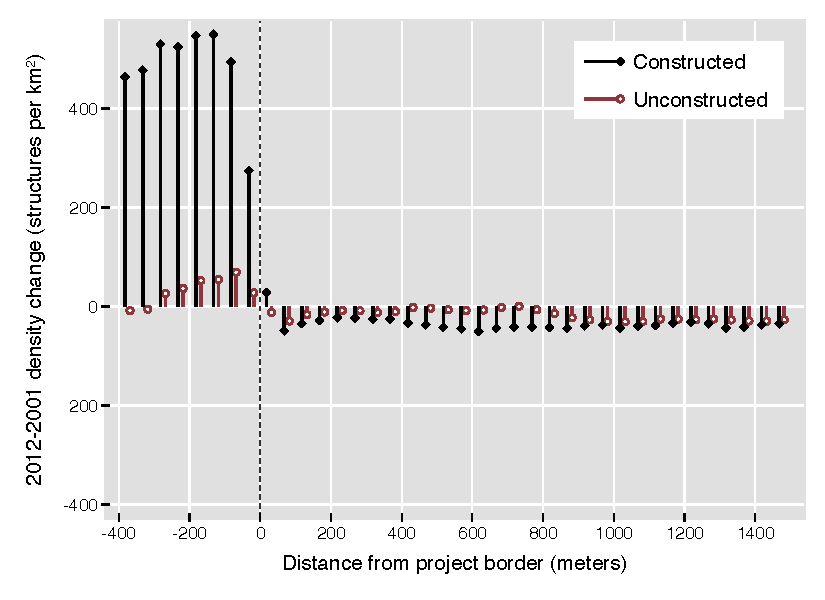
\includegraphics[width=\textwidth,trim={0.3cm .3cm 0.1cm 0cm}, clip=true]{figures/bblu_for_fe_rawchanges_4_mp_postk.pdf}

        \end{subfigure}
        \hfill
        \begin{subfigure}[b]{0.48\textwidth}  
                    \caption[]%
            {{\footnotesize \textbf{All Projects} changes informal  fe }}      
            \label{fig:preinf}
            \centering 
            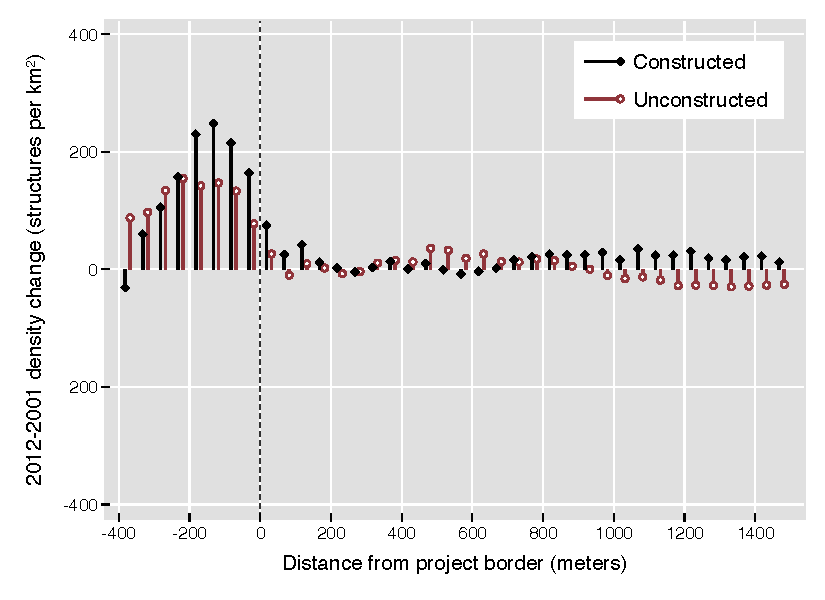
\includegraphics[width=\textwidth,trim={0.3cm .3cm 0.1cm 0cm}, clip=true]{figures/bblu_inf_fe_rawchanges_4_mp_postk.pdf}

        \end{subfigure}
        \begin{subfigure}[b]{0.48\textwidth}
                    \caption[Network2]%
            {{\footnotesize \textbf{Greenfield} changes formal  fe}}    
            \label{fig:prefor}
            \centering
            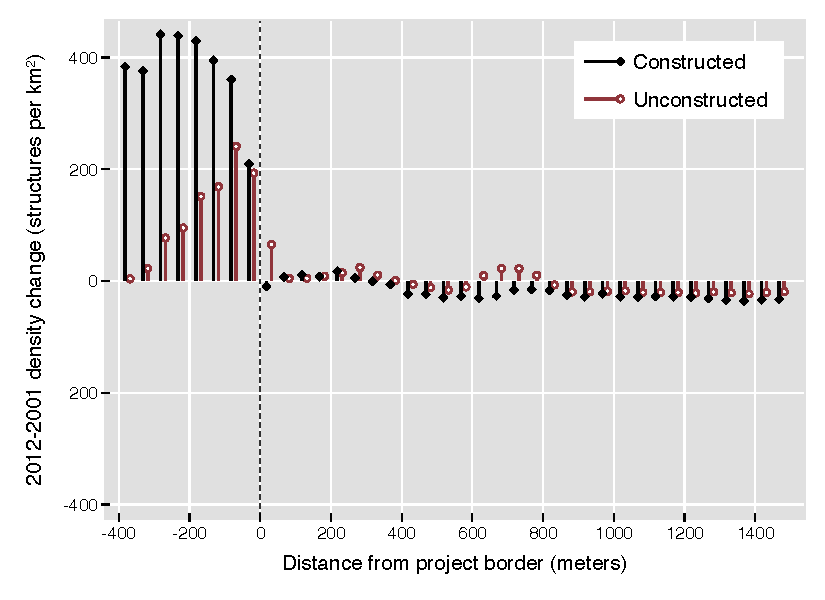
\includegraphics[width=\textwidth,trim={0.3cm .3cm 0.1cm 0cm}, clip=true]{figures/bblu_for_fe_rawchanges_4_1_mp_postk.pdf}

        \end{subfigure}
        \hfill
        \begin{subfigure}[b]{0.48\textwidth}  
                    \caption[]%
            {{\footnotesize \textbf{Greenfield} changes informal fe}}     
            \label{fig:preinf}
            \centering 
            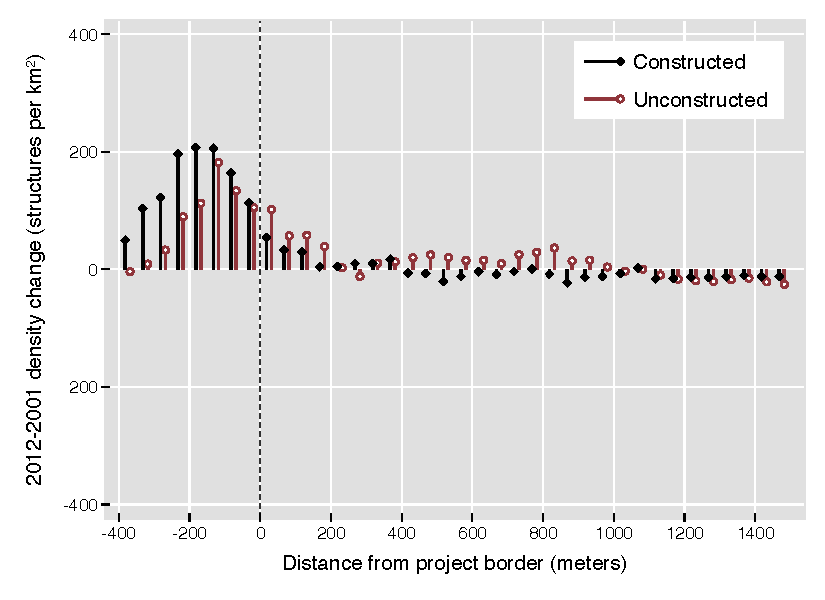
\includegraphics[width=\textwidth,trim={0.3cm .3cm 0.1cm 0cm}, clip=true]{figures/bblu_inf_fe_rawchanges_4_1_mp_postk.pdf}

        \end{subfigure}
        \begin{subfigure}[b]{0.48\textwidth}
                    \caption[Network2]%
            {{\footnotesize \textbf{In-Situ} changes formal fe}}   
            \label{fig:prefor}
            \centering
            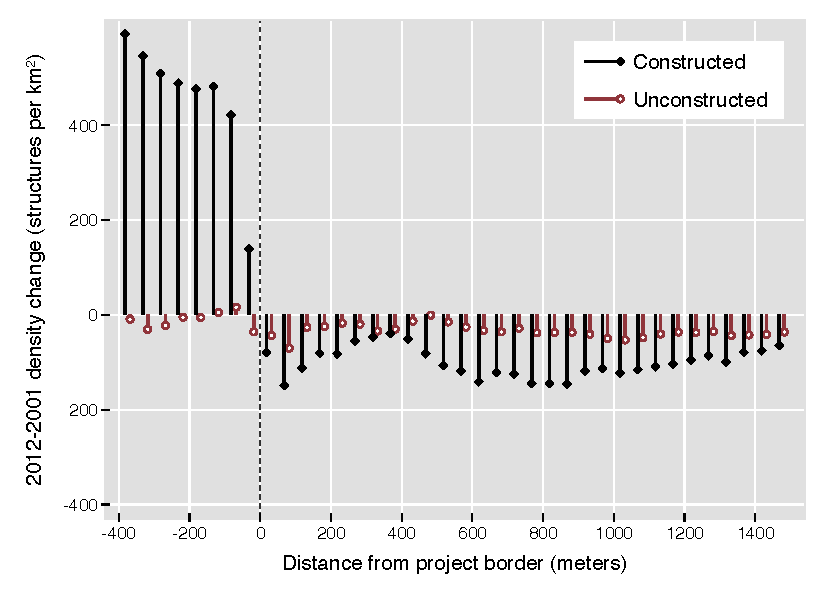
\includegraphics[width=\textwidth,trim={0.3cm .3cm 0.1cm 0cm}, clip=true]{figures/bblu_for_fe_rawchanges_4_2_mp_postk.pdf}

        \end{subfigure}
        \hfill
        \begin{subfigure}[b]{0.48\textwidth}  
                    \caption[]%
            {{\footnotesize \textbf{In-Situ} changes informal fe}}     
            \label{fig:preinf}
            \centering 
            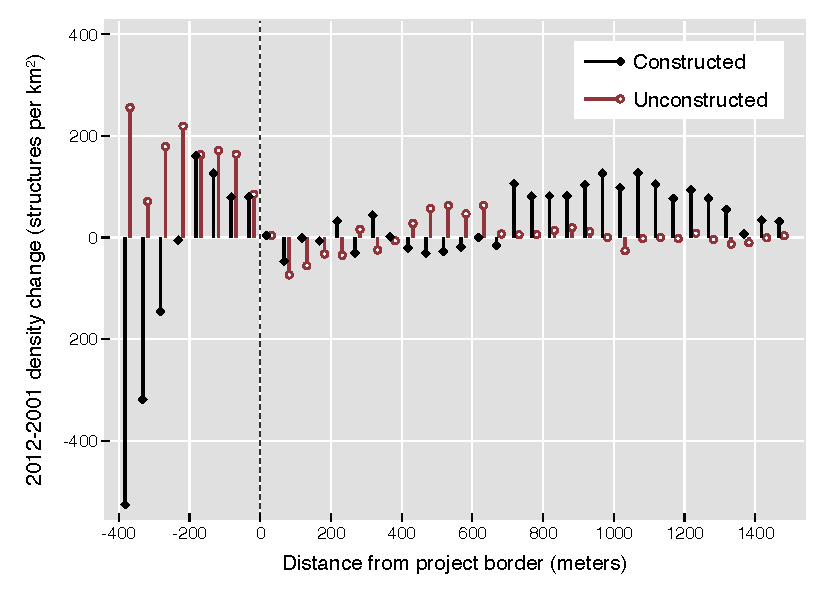
\includegraphics[width=\textwidth,trim={0.3cm .3cm 0.1cm 0cm}, clip=true]{figures/bblu_inf_fe_rawchanges_4_2_mp_postk.pdf}

        \end{subfigure}
        \begin{subfigure}[b]{0.48\textwidth}
                    \caption[Network2]%
            {{\footnotesize \textbf{Other} changes formal fe}}   
            \label{fig:prefor}
            \centering
            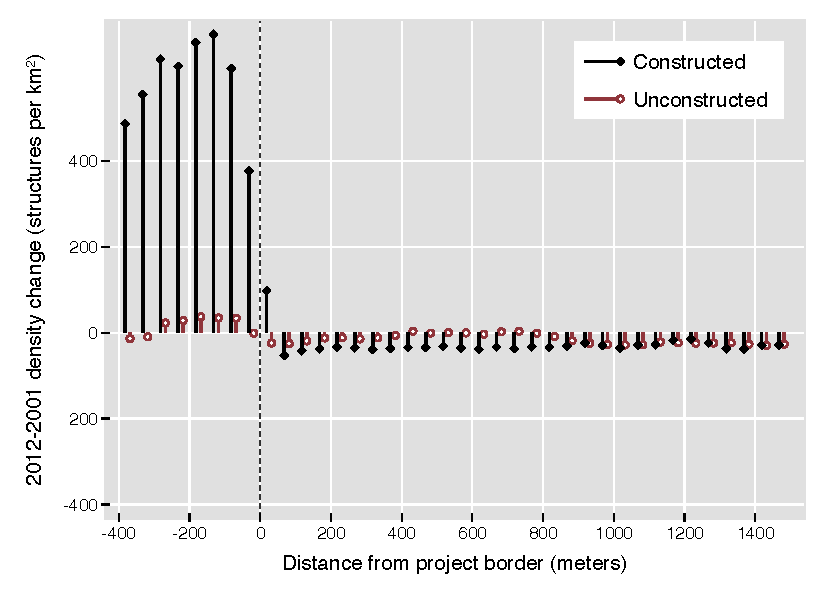
\includegraphics[width=\textwidth,trim={0.3cm .3cm 0.1cm 0cm}, clip=true]{figures/bblu_for_fe_rawchanges_4_3_mp_postk.pdf}

        \end{subfigure}
        \hfill
        \begin{subfigure}[b]{0.48\textwidth} 
                    \caption[]%
            {{\footnotesize \textbf{Other} changes informal  fe}}      
            \label{fig:preinf} 
            \centering 
            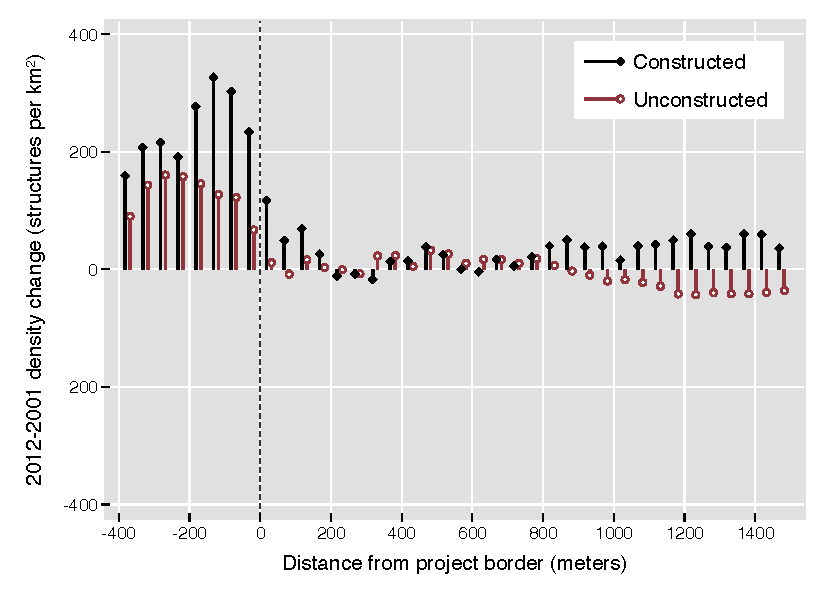
\includegraphics[width=\textwidth,trim={0.3cm .3cm 0.1cm 0cm}, clip=true]{figures/bblu_inf_fe_rawchanges_4_3_mp_postk.pdf}

        \end{subfigure}
\end{figure*}







\begin{table}
\caption{Building Density}
\begin{tabular}{lDDDDD}
\toprule
 & \small (1) & \small (2)  & \small (3) & \small (4) & \small (5) \\
 & Total & Formal  & Informal & Informal Bkyd. & Informal Non-Bkyd. \\ \midrule
\textbf{All Projects} \\inside project      &     548.268\textsuperscript{a}&     534.970\textsuperscript{a}&      13.298                   &     391.907\textsuperscript{a}&    -378.609\textsuperscript{a}\\
                    &   (122.989)                   &    (71.175)                   &    (95.954)                   &    (86.437)                   &    (82.246)                   \\[0.5em]
0-300m outside project &      25.895                   &      33.553                   &      -7.658                   &      25.114                   &     -32.772                   \\
                    &    (42.051)                   &    (25.718)                   &    (33.128)                   &    (31.798)                   &    (28.987)                   \\[0.5em]
300-600m outside project &     -38.898                   &       2.988                   &     -41.886\textsuperscript{c}&     -23.046                   &     -18.841                   \\
                    &    (30.409)                   &    (16.840)                   &    (24.534)                   &    (22.309)                   &    (18.137)                   \\[0.5em]
R$^2$               &       0.349                   &       0.288                   &       0.276                   &       0.265                   &       0.147                   \\

\midrule
\textbf{Greenfield} \\   inside project      &     307.366                   &     253.793\textsuperscript{c}&      53.573                   &      98.627                   &     -45.054                   \\
                    &   (206.153)                   &   (139.113)                   &    (97.167)                   &    (99.431)                   &    (55.228)                   \\[0.01em]
0-300m outside project &     -55.865                   &     -31.482                   &     -24.383                   &     -52.861                   &      28.478                   \\
                    &    (87.987)                   &    (45.832)                   &    (57.134)                   &    (44.432)                   &    (50.864)                   \\[0.01em]
300-600m outside project&     -65.896                   &     -28.884                   &     -37.012                   &     -31.613\textsuperscript{c}&      -5.398                   \\
                    &    (45.127)                   &    (22.852)                   &    (28.716)                   &    (16.289)                   &    (21.978)                   \\[0.8em] 
\textbf{In-Situ Upgrading} \\   inside project      &     297.320                   &     740.828\textsuperscript{a}&    -443.508                   &     291.123                   &    -734.631\textsuperscript{a}\\
                    &   (449.822)                   &   (171.354)                   &   (329.831)                   &   (349.258)                   &   (254.964)                   \\[0.01em]
0-300m outside project &      46.826                   &     121.333                   &     -74.508                   &     -32.652                   &     -41.856                   \\
                    &   (158.212)                   &   (103.229)                   &    (99.435)                   &   (144.122)                   &   (106.493)                   \\[0.01em]
300-600m outside project &       6.707                   &     109.943                   &    -103.236                   &     -91.058                   &     -12.178                   \\
                    &    (96.146)                   &    (68.737)                   &    (66.675)                   &    (84.258)                   &    (77.639)                   \\[0.8em]
\textbf{Other} \\   inside project      &     803.411\textsuperscript{a}&     652.679\textsuperscript{a}&     150.733                   &     609.015\textsuperscript{a}&    -458.283\textsuperscript{a}\\
                    &   (152.730)                   &    (73.201)                   &   (121.740)                   &   (102.106)                   &    (99.714)                   \\[0.01em]
0-300m outside project &      17.149                   &      28.704                   &     -11.555                   &      41.144                   &     -52.698                   \\
                    &    (66.198)                   &    (28.716)                   &    (56.588)                   &    (42.039)                   &    (34.967)                   \\[0.01em]
300-600m outside project &     -70.257                   &     -20.255                   &     -50.002                   &     -13.392                   &     -36.609\textsuperscript{c}\\
                    &    (45.095)                   &    (20.521)                   &    (38.851)                   &    (33.319)                   &    (20.567)                   \\[0.8em]
Mean Outcome 2001   &      379.90                   &      203.91                   &      175.98                   &       66.26                   &      109.72                   \\
Mean Outcome 2011   &      584.70                   &      281.66                   &      303.04                   &      192.77                   &      110.27                   \\
R$^2$               &       0.354                   &       0.290                   &       0.284                   &       0.268                   &       0.158                   \\
N                   &   2,721,910                   &   2,721,910                   &   2,721,910                   &   2,721,910                   &   2,721,910                   \\

\bottomrule
\end{tabular}
\end{table}





\begin{table}[h!] 
\caption{Effect of Housing Projects on Socio-demographics}
\label{table:sorting}
\small
\centering
%\caption{Census Composition Estimates }
\vspace{-2mm}
\begin{tabular}{lDDDDD}
\toprule
& \small (1) & \small (2) & \small (3) & \small (4)& \small (5)\\
& \small Age & \small P.O.B. not Gauteng & \small Unemployed & \small Years of Education & \small Monthly Income \\ \midrule 
\textbf{All Projects} \\inside project      &       0.332                   &      -0.017                   &      -0.006                   &       0.241\textsuperscript{c}&    1684.522\textsuperscript{a}\\
                    &     (0.389)                   &     (0.027)                   &     (0.019)                   &     (0.133)                   &   (530.080)                   \\[0.5em]
0-300m outside project &       0.521                   &       0.019                   &       0.016                   &       0.174                   &    1159.925\textsuperscript{b}\\
                    &     (0.344)                   &     (0.018)                   &     (0.019)                   &     (0.123)                   &   (503.517)                   \\[0.5em]
300-600m outside project &      -0.102                   &       0.012                   &       0.014                   &       0.046                   &     709.583                   \\
                    &     (0.344)                   &     (0.017)                   &     (0.015)                   &     (0.101)                   &   (476.879)                   \\[0.5em]
R$^2$               &       0.334                   &       0.475                   &       0.343                   &       0.502                   &       0.341                   \\

\midrule
\textbf{Greenfield} \\   inside project      &      -0.721                   &      -0.016                   &       0.053                   &      -0.017                   &     871.394                   \\
                    &     (0.869)                   &     (0.056)                   &     (0.050)                   &     (0.329)                   &   (992.013)                   \\[0.01em]
0-300m outside project &      -0.339                   &       0.040                   &       0.005                   &       0.129                   &     579.393                   \\
                    &     (0.723)                   &     (0.025)                   &     (0.042)                   &     (0.236)                   &   (763.926)                   \\[0.01em]
300-600m outside project&      -1.188\textsuperscript{c}&       0.053                   &       0.053                   &       0.279                   &    -287.480                   \\
                    &     (0.681)                   &     (0.034)                   &     (0.033)                   &     (0.229)                   &   (756.262)                   \\[0.8em] 
\textbf{In-Situ Upgrading} \\   inside project      &       0.523                   &      -0.037                   &      -0.030                   &       0.121                   &    1205.487                   \\
                    &     (0.737)                   &     (0.032)                   &     (0.027)                   &     (0.258)                   &  (1298.170)                   \\[0.01em]
0-300m outside project &       0.169                   &      -0.033                   &       0.014                   &       0.281                   &    1015.708                   \\
                    &     (0.694)                   &     (0.026)                   &     (0.028)                   &     (0.276)                   &  (1314.290)                   \\[0.01em]
300-600m outside project &      -1.073                   &       0.015                   &       0.030                   &      -0.276                   &   -1047.475                   \\
                    &     (0.774)                   &     (0.028)                   &     (0.028)                   &     (0.241)                   &  (1147.813)                   \\[0.8em]
\textbf{Other} \\   inside project      &       0.569                   &       0.028                   &      -0.014                   &       0.299                   &    2459.343\textsuperscript{a}\\
                    &     (0.618)                   &     (0.036)                   &     (0.027)                   &     (0.193)                   &   (763.887)                   \\[0.01em]
0-300m outside project &       1.069\textsuperscript{c}&       0.039                   &       0.006                   &       0.147                   &    1628.903\textsuperscript{b}\\
                    &     (0.574)                   &     (0.028)                   &     (0.029)                   &     (0.160)                   &   (691.905)                   \\[0.01em]
300-600m outside project &       0.757                   &       0.007                   &      -0.011                   &       0.121                   &    1906.369\textsuperscript{a}\\
                    &     (0.551)                   &     (0.028)                   &     (0.023)                   &     (0.157)                   &   (665.807)                   \\[0.8em]
Mean Outcome 2001   &       27.30                   &        0.37                   &        0.47                   &        8.26                   &    2,475.96                   \\
Mean Outcome 2011   &       28.30                   &        0.43                   &        0.33                   &        9.68                   &    4,486.48                   \\
R$^2$               &       0.340                   &       0.489                   &       0.347                   &       0.507                   &       0.346                   \\
N                   &      12,733                   &      12,726                   &      12,723                   &      12,727                   &      12,723                   \\

\bottomrule
\multicolumn{6}{l}{\footnotesize Standard errors clustered at the project level in parenthesis. \textsuperscript{c} p$<$0.10, \textsuperscript{b} p$<$0.05, \textsuperscript{a} p$<$0.01  }\\
\multicolumn{6}{l}{\footnotesize P.O.B. means ``place of birth.''  Monthly income is in Rands.}
\end{tabular}
\end{table}








\begin{landscape}
{\footnotesize

\begin{table}[]
\small
\centering
\caption{Census Household-level Estimates }\label{table:censusestimates}
\vspace{-2mm}
\resizebox{.9\linewidth}{!}{
\begin{tabular}{lDDDDDDDD}
\toprule
 & \small (1) & \small (2)  & \small (3) & \small (4) & \small (5)  & \small (6)  & \small (7) & (8)\\
 & \small Flush Toilet & \small Water Indoors  & \small Electricity Cooking & \small Electricity Heating & \small Electricity Lighting  & \small Number of Rooms  & \small Household Size & Population Density\\ \midrule 
\textbf{All Projects} \\inside project      &       0.105                   &       0.193\textsuperscript{a}&       0.180\textsuperscript{b}&       0.165\textsuperscript{b}&       0.123                   &       0.210                   &       0.077                   &   -1166.752                   \\
                    &     (0.074)                   &     (0.044)                   &     (0.082)                   &     (0.080)                   &     (0.085)                   &     (0.169)                   &     (0.098)                   &   (916.987)                   \\[0.5em]
0-300m outside project &      -0.011                   &       0.051                   &       0.004                   &       0.014                   &      -0.017                   &       0.088                   &      -0.021                   &    -538.243                   \\
                    &     (0.039)                   &     (0.040)                   &     (0.037)                   &     (0.039)                   &     (0.036)                   &     (0.130)                   &     (0.059)                   &   (657.864)                   \\[0.5em]
300-600m outside project &      -0.003                   &       0.046                   &       0.005                   &       0.017                   &      -0.003                   &      -0.041                   &      -0.014                   &   -1131.608                   \\
                    &     (0.029)                   &     (0.034)                   &     (0.028)                   &     (0.031)                   &     (0.027)                   &     (0.119)                   &     (0.056)                   &   (843.274)                   \\[0.5em]
R$^2$               &       0.230                   &       0.293                   &       0.324                   &       0.338                   &       0.242                   &       0.296                   &       0.340                   &       0.409                   \\

\midrule
\textbf{Greenfield} \\   inside project      &       0.062                   &       0.259\textsuperscript{c}&       0.068                   &       0.026                   &       0.033                   &       0.360                   &       0.155                   &      96.822                   \\
                    &     (0.159)                   &     (0.138)                   &     (0.125)                   &     (0.135)                   &     (0.118)                   &     (0.516)                   &     (0.239)                   &  (3723.521)                   \\[0.01em]
0-300m outside project &      -0.086                   &       0.095                   &      -0.052                   &      -0.023                   &      -0.088                   &       0.380                   &       0.201                   &    -435.481                   \\
                    &     (0.085)                   &     (0.089)                   &     (0.059)                   &     (0.063)                   &     (0.060)                   &     (0.289)                   &     (0.149)                   &  (1894.832)                   \\[0.01em]
300-600m outside project&      -0.015                   &       0.001                   &      -0.015                   &      -0.013                   &      -0.007                   &      -0.278                   &      -0.062                   &   -1721.429                   \\
                    &     (0.066)                   &     (0.067)                   &     (0.048)                   &     (0.060)                   &     (0.048)                   &     (0.236)                   &     (0.117)                   &  (2682.519)                   \\[0.8em] 
\textbf{In-Situ Upgrading} \\   inside project      &       0.331\textsuperscript{b}&       0.125                   &       0.155                   &       0.186\textsuperscript{b}&       0.157\textsuperscript{c}&       0.562\textsuperscript{b}&       0.335\textsuperscript{b}&   -2380.173                   \\
                    &     (0.142)                   &     (0.091)                   &     (0.097)                   &     (0.089)                   &     (0.093)                   &     (0.261)                   &     (0.137)                   &  (1799.177)                   \\[0.01em]
0-300m outside project &       0.072                   &       0.038                   &       0.044                   &       0.057                   &       0.012                   &       0.057                   &       0.149                   &   -1263.682                   \\
                    &     (0.084)                   &     (0.090)                   &     (0.071)                   &     (0.079)                   &     (0.068)                   &     (0.299)                   &     (0.092)                   &  (1172.774)                   \\[0.01em]
300-600m outside project &      -0.008                   &      -0.006                   &       0.007                   &       0.048                   &      -0.045                   &      -0.332                   &       0.038                   &     784.643                   \\
                    &     (0.064)                   &     (0.077)                   &     (0.073)                   &     (0.077)                   &     (0.065)                   &     (0.338)                   &     (0.091)                   &  (1089.242)                   \\[0.8em]
\textbf{Other} \\   inside project      &      -0.034                   &       0.198\textsuperscript{a}&       0.147                   &       0.121                   &       0.066                   &      -0.049                   &      -0.145                   &   -1487.616                   \\
                    &     (0.093)                   &     (0.061)                   &     (0.116)                   &     (0.111)                   &     (0.124)                   &     (0.253)                   &     (0.127)                   &  (1111.727)                   \\[0.01em]
0-300m outside project &      -0.031                   &       0.068                   &      -0.004                   &       0.001                   &      -0.009                   &       0.143                   &      -0.158\textsuperscript{c}&    -855.566                   \\
                    &     (0.045)                   &     (0.055)                   &     (0.049)                   &     (0.050)                   &     (0.049)                   &     (0.181)                   &     (0.086)                   &   (993.261)                   \\[0.01em]
300-600m outside project &       0.005                   &       0.092\textsuperscript{c}&       0.019                   &       0.025                   &       0.023                   &       0.173                   &      -0.066                   &   -2099.109\textsuperscript{c}\\
                    &     (0.039)                   &     (0.052)                   &     (0.040)                   &     (0.040)                   &     (0.039)                   &     (0.167)                   &     (0.091)                   &  (1091.440)                   \\[0.8em]
Mean Outcome 2001   &        0.79                   &        0.35                   &        0.66                   &        0.62                   &        0.77                   &        3.30                   &        3.51                   &    8,566.83                   \\
Mean Outcome 2011   &        0.83                   &        0.54                   &        0.81                   &        0.72                   &        0.82                   &        3.56                   &        3.18                   &    9,823.82                   \\
R$^2$               &       0.249                   &       0.309                   &       0.342                   &       0.353                   &       0.265                   &       0.304                   &       0.353                   &       0.418                   \\
N                   &      12,732                   &      12,732                   &      12,732                   &      12,732                   &      12,732                   &      12,709                   &      12,730                   &      12,734                   \\

\bottomrule
\multicolumn{9}{l}{\footnotesize All regressions include 3km grid Fixed-Effects. Standard errors clustered at the project level in parenthesis. \textsuperscript{c} p$<$0.10,\textsuperscript{b} p$<$0.05,\textsuperscript{a} p$<$0.01 }
\end{tabular}
}
\end{table}

}
\end{landscape}




\begin{table}
\small
\centering
\caption{Triple Difference Estimates on Log-Prices}\label{table:priceDDD_het}
\vspace{-2mm}
\begin{tabular}{lCC}
\toprule
 & \small (1) & \small (2)  \\ \midrule 
 \textbf{All Projects} \\
 inside project      &      -0.261                   &      -0.253                   \\
                    &     (0.349)                   &     (0.349)                   \\[0.55em]
0-300m outside project &      -0.103                   &      -0.100                   \\
                    &     (0.148)                   &     (0.148)                   \\[0.5em]
300-600m outside project &      -0.101                   &      -0.098                   \\
                    &     (0.099)                   &     (0.099)                   \\[0.5em]
Lot Size Controls   &                               &  \checkmark                   \\
r2                  &        0.34                   &        0.34                   \\
N                   &      67,751                   &      67,751                   \\

 \midrule
\textbf{Greenfield} \\   inside project      &       0.216                   &       0.210                   \\
                    &     (0.233)                   &     (0.232)                   \\[0.01em]
0-300m outside project &      -0.011                   &       0.000                   \\
                    &     (0.196)                   &     (0.195)                   \\[0.01em]
300-600m outside project&       0.038                   &       0.045                   \\
                    &     (0.164)                   &     (0.165)                   \\[0.8em]
\textbf{In-Situ Upgrading} \\   inside project      &      -0.220                   &      -0.202                   \\
                    &     (0.433)                   &     (0.436)                   \\[0.01em]
0-300m outside project &      -0.548\textsuperscript{c}&      -0.548\textsuperscript{c}\\
                    &     (0.316)                   &     (0.315)                   \\[0.01em]
300-600m outside project &      -0.450\textsuperscript{b}&      -0.450\textsuperscript{b}\\
                    &     (0.223)                   &     (0.223)                   \\[0.8em]
\textbf{Other} \\   inside project      &      -0.976\textsuperscript{b}&      -0.972\textsuperscript{b}\\
                    &     (0.409)                   &     (0.408)                   \\[0.01em]
0-300m outside project &      -0.216                   &      -0.214                   \\
                    &     (0.170)                   &     (0.170)                   \\[0.01em]
300-600m outside project &      -0.195                   &      -0.195                   \\
                    &     (0.125)                   &     (0.125)                   \\[0.8em]
Lot Size Controls   &                               &  \checkmark                   \\
r2                  &        0.35                   &        0.35                   \\
N                   &      67,751                   &      67,751                   \\

\bottomrule
\multicolumn{3}{l}{\footnotesize Standard errors clustered at the project level in parenthesis.} \\
\multicolumn{3}{l}{ \textsuperscript{c} p$<$0.10,\textsuperscript{b} p$<$0.05,\textsuperscript{a} p$<$0.01 }
\end{tabular}
\end{table} 

% \begin{figure}
% 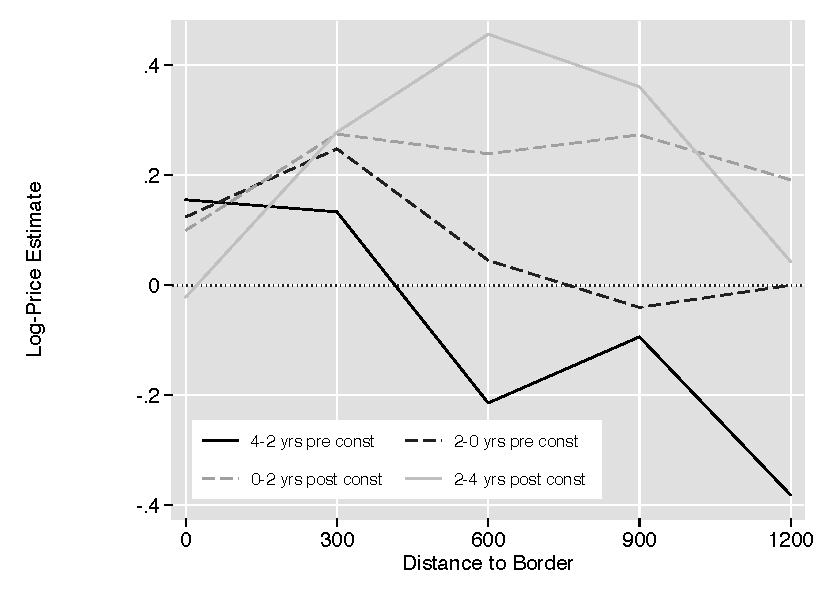
\includegraphics{figures/price_to_event_30.pdf}
% \end{figure}


\end{document}


